\documentclass[12pt, oneside]{article}   	
\usepackage[margin=1in]{geometry}
\geometry{letterpaper}

\usepackage{fontspec}
\setmainfont{Times New Roman} 
\setmonofont{Consolas}             		
       		
%\usepackage[parfill]{parskip}    		
\usepackage{graphicx}	
\usepackage{amssymb}
\usepackage{array}
\usepackage{caption}
 \usepackage[labelformat=empty]{caption}
 
\usepackage{listings}
\usepackage{color}

\definecolor{dkgreen}{rgb}{0,0.6,0}
\definecolor{gray}{rgb}{0.5,0.5,0.5}
\definecolor{mauve}{rgb}{0.58,0,0.82}

\makeatletter
\newcommand{\srcsize}{\@setfontsize{\srcsize}{10pt}{10pt}}
\makeatother

\lstset{frame=tb,
  language=SQL,
  %aboveskip=3mm,
  %belowskip=3mm,
  basicstyle=\srcsize,
  showstringspaces=false,
  columns=flexible,
  basicstyle={\srcsize\ttfamily},
  numbers=none,
  numberstyle=\tiny\color{gray},
  keywordstyle=\color{mauve},
  commentstyle=\color{dkgreen},
  stringstyle=\color{blue},
  breaklines=true,
  breakatwhitespace=true,
  tabsize=2
}

\usepackage{titling}

\setlength{\droptitle}{-5em}

\title{JDBC Assessment}
\author{Paul McHard - 2085227M} 
\date{\today}					

\begin{document}
\maketitle
\subsubsection*{State of Program}
The program has been completed as required by the specification and achieves the desired functionality. The GUI is clearly layout and easy to read; the program is capable of displaying the desired information regarding courses, their instructors and capacities in one report, and information on members and the courses to which they are enrolled on another report. The program also allows members to be booked onto a course and updates the database accordingly, as well as preventing certain bookings in the case where the user is already booked onto the course or if the course is already fully booked.
\subsubsection*{SQL Queries used}
The program was designed to place more of the key data processing work on the shoulders of Java rather than SQL. This is reflected in the code as more complex systems; use of objects, if statements  and nested looping to check inputs and data validity, are used in the program to deliver the necessary functionality. As the Java code handles the majority of this data processing, the SQL code is left with only interactions with the database; simple extraction and insertion of data into the relevant tables, as opposed to handling more specialised requests of the database and selection using more complex SQL statements, potentially involving nesting, joins or specifying criterion.
\subsubsection*{Code Examples}
\lstinputlisting[language=SQL]{SQLExample.sql}
\subsubsection*{Testing Performed}
\begin{center}
\begin{tabular}{ | m{12cm} | m{4cm} | } 
 \hline
 \textbf{Test} & \textbf{Appendix Figure} \\ 
  \hline
Program produces list of all courses, their instructors, capacities and current enrollment. & 1 \\ 
  \hline
 Program produces list all members currently booked on a course, their names, ID's and the course their booked on. & 2 \\ 
 \hline
 Program allows a user to be booked onto a course & 3,4 \\
 \hline
 Program prevents a booking for a course which is at capacity & 5 \\
 \hline
 Program prevents a booking if user is already booked on course & 6 \\
 \hline
\end{tabular}
\end{center}
\subsubsection*{Conclusion}
There was concern during development that this Java-centric approach, while successful, was inappropriate and missed the core learning objectives of the task. However, on discussion of this with the course head, it was determined that the specification facilitated many possible approaches, so this is perfectly valid. There is an argument for this method from a technical perspective; by performing all data processing and input checking in the Java code, the system is safer and more secure at dealing with invalid, potentially damaging database commands, as more rigorous design can be used to catch such instructions and prevent corruption of the database.\newline \newline
One key thing I have learned is that there is a large degree of freedom afforded by a project which involves the interaction of an object oriented language like Java and a database utilising a SQL, in terms of what prevalence is put on either language for development. These design decisions are important and, for a professional program, careful attention should be given to determine the best mix of Java and SQL to achieve the desired functionality and maintain a secure program and database.
\newpage
\subsubsection*{Appendix - Testing Screenshots}
\begin{figure}[ht!]
\centering
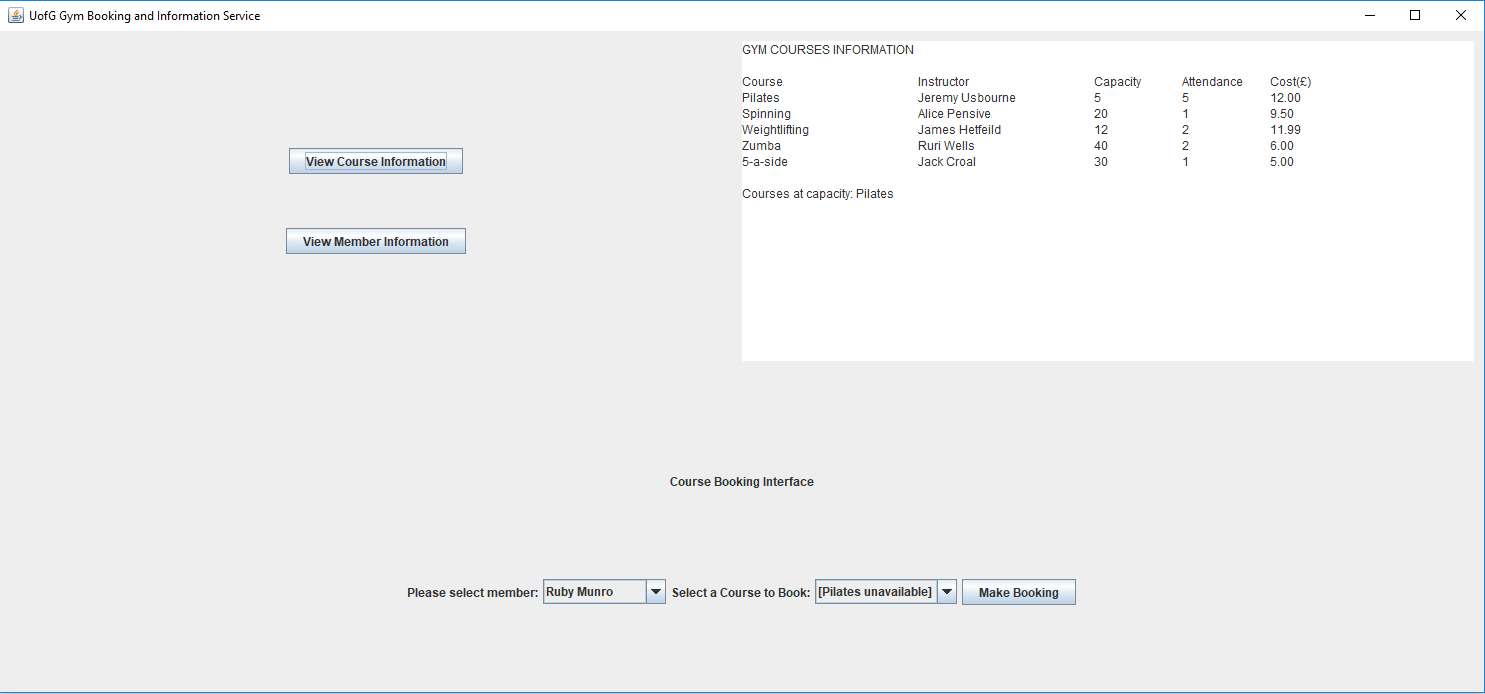
\includegraphics[width=17cm]{fig1}
\caption{\textit{Figure 1}}
\end{figure}
\begin{figure}[ht!]
\centering
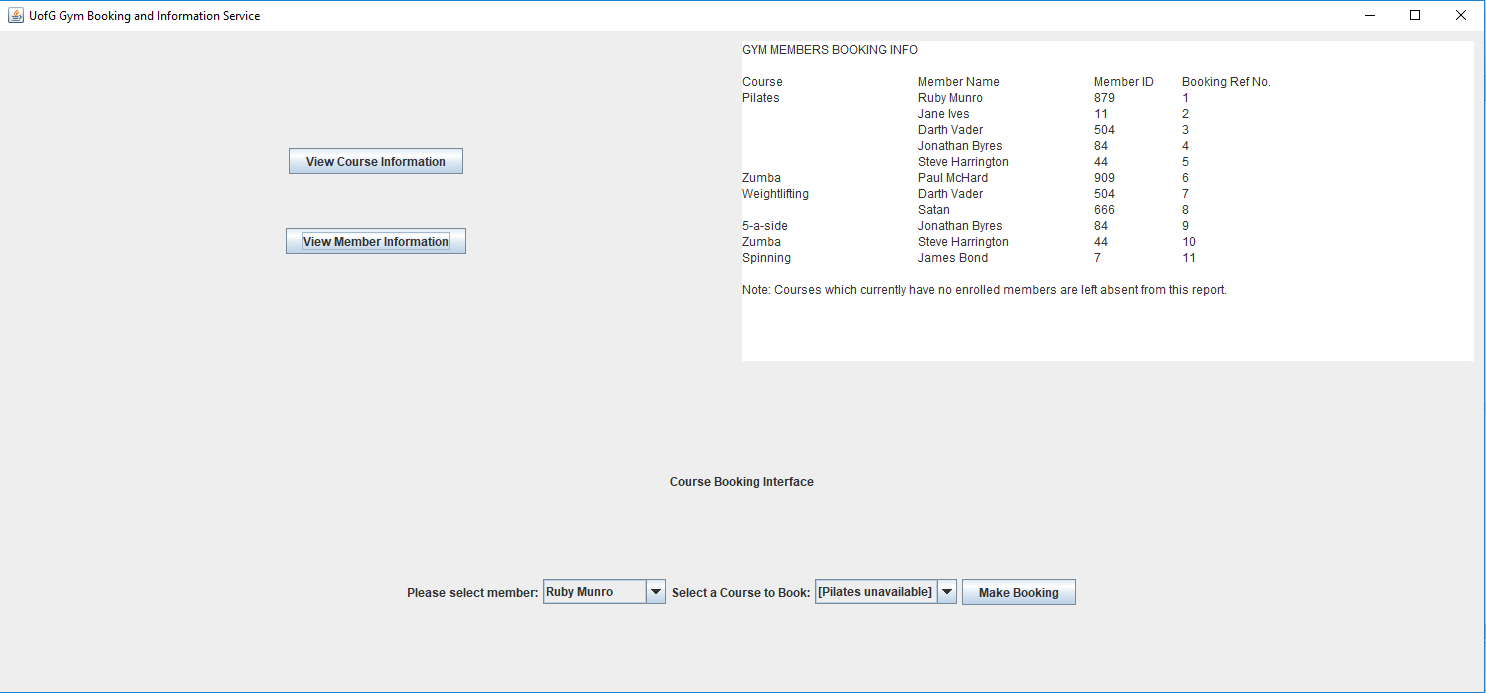
\includegraphics[width=17cm]{fig2}
\caption*{ \textit{Figure 2} }
\end{figure}
\begin{figure}[ht!]
\centering
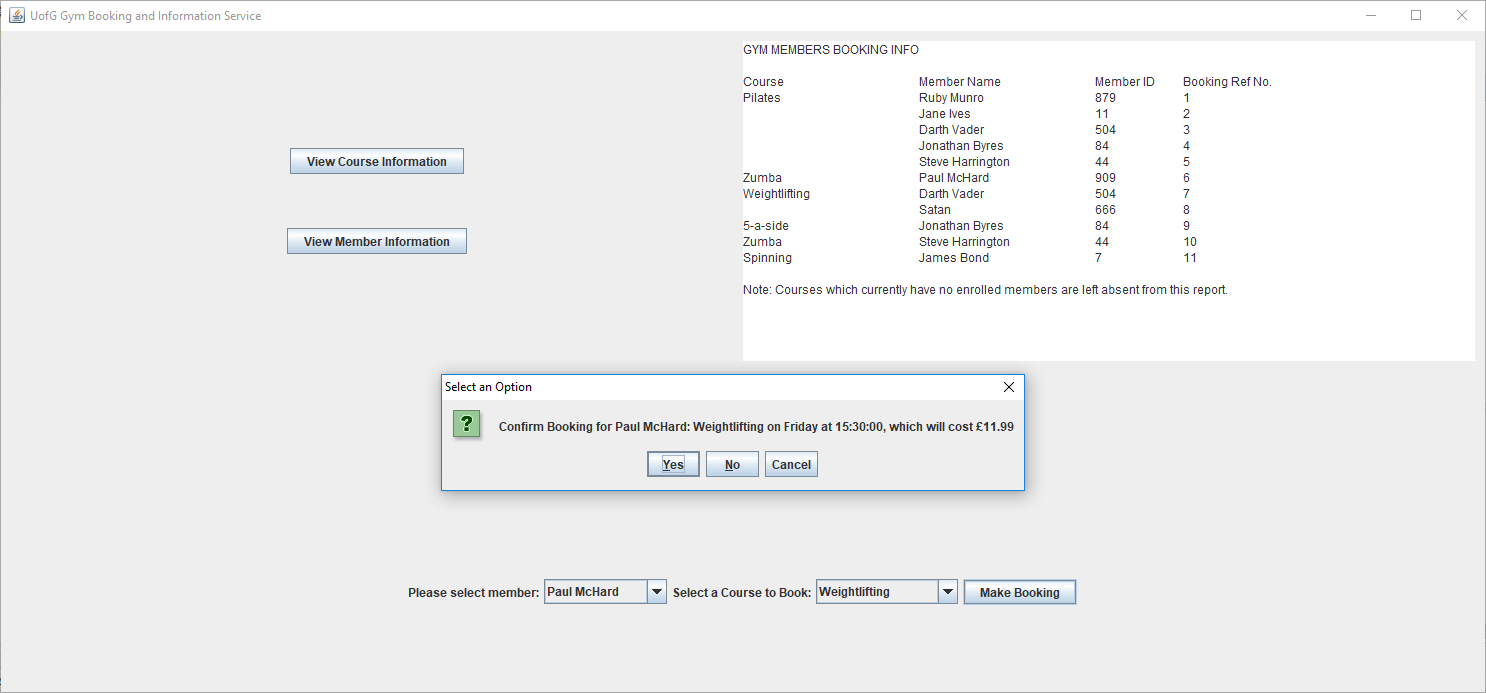
\includegraphics[width=17cm]{fig4}
\caption*{ \textit{Figure 3} }
\end{figure}
\begin{figure}[ht!]
\centering
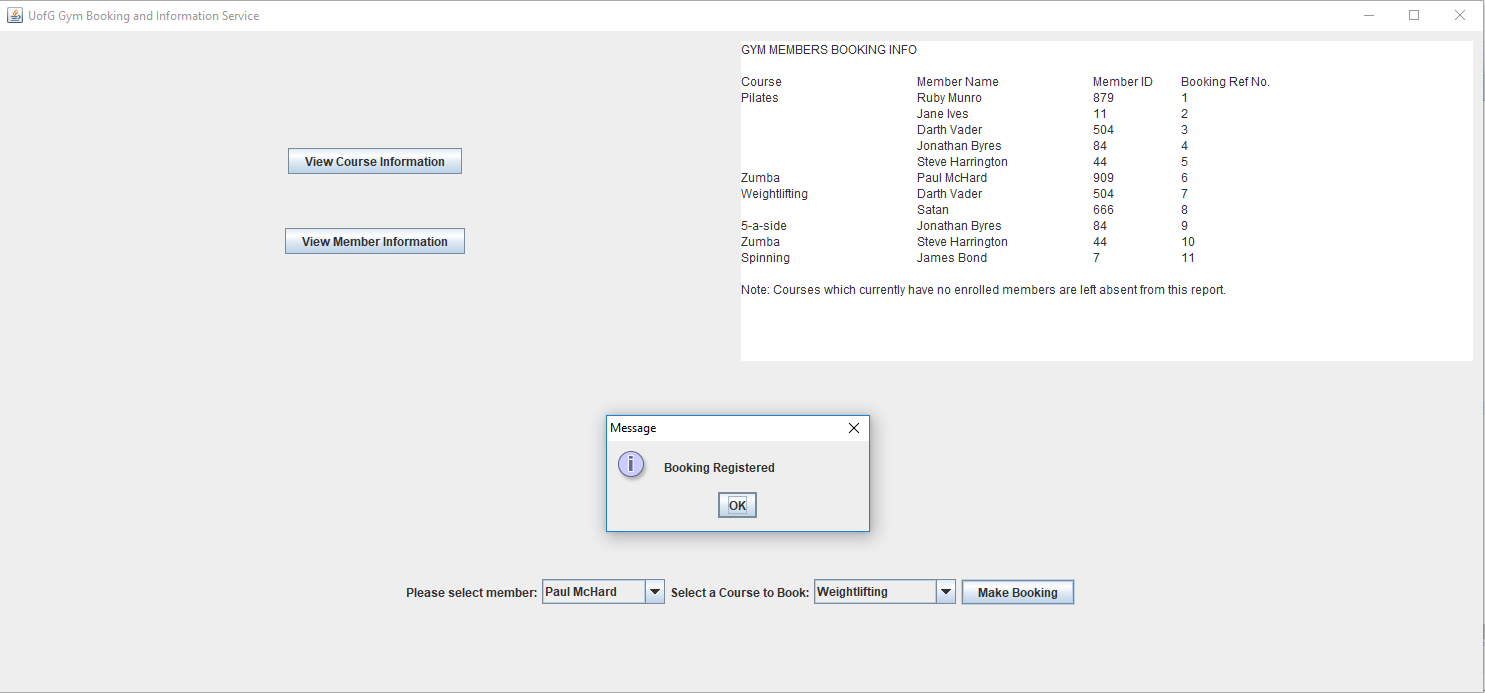
\includegraphics[width=17cm]{fig5}
\caption*{ \textit{Figure 4} }
\end{figure}
\begin{figure}[ht!]
\centering
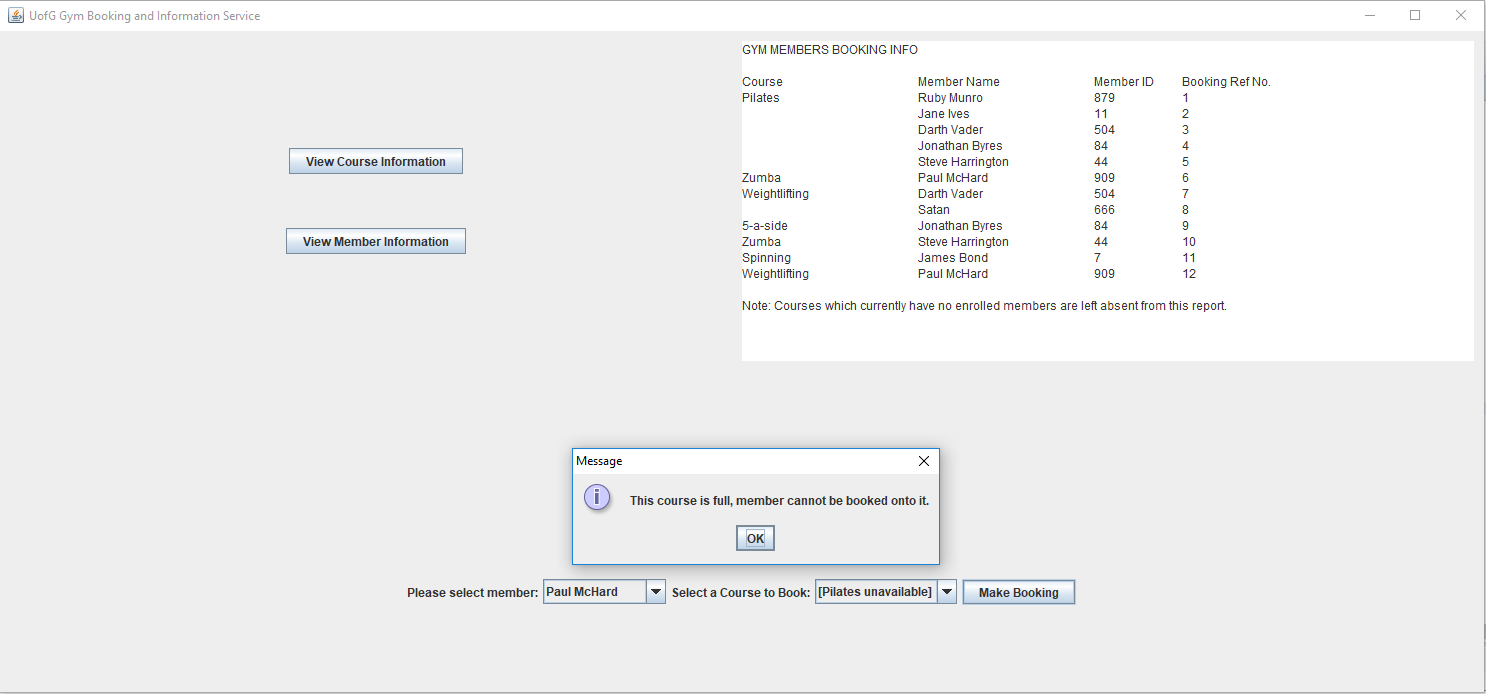
\includegraphics[width=17cm]{fig8}
\caption*{ \textit{Figure 5} }
\end{figure}
\begin{figure}[ht!]
\centering
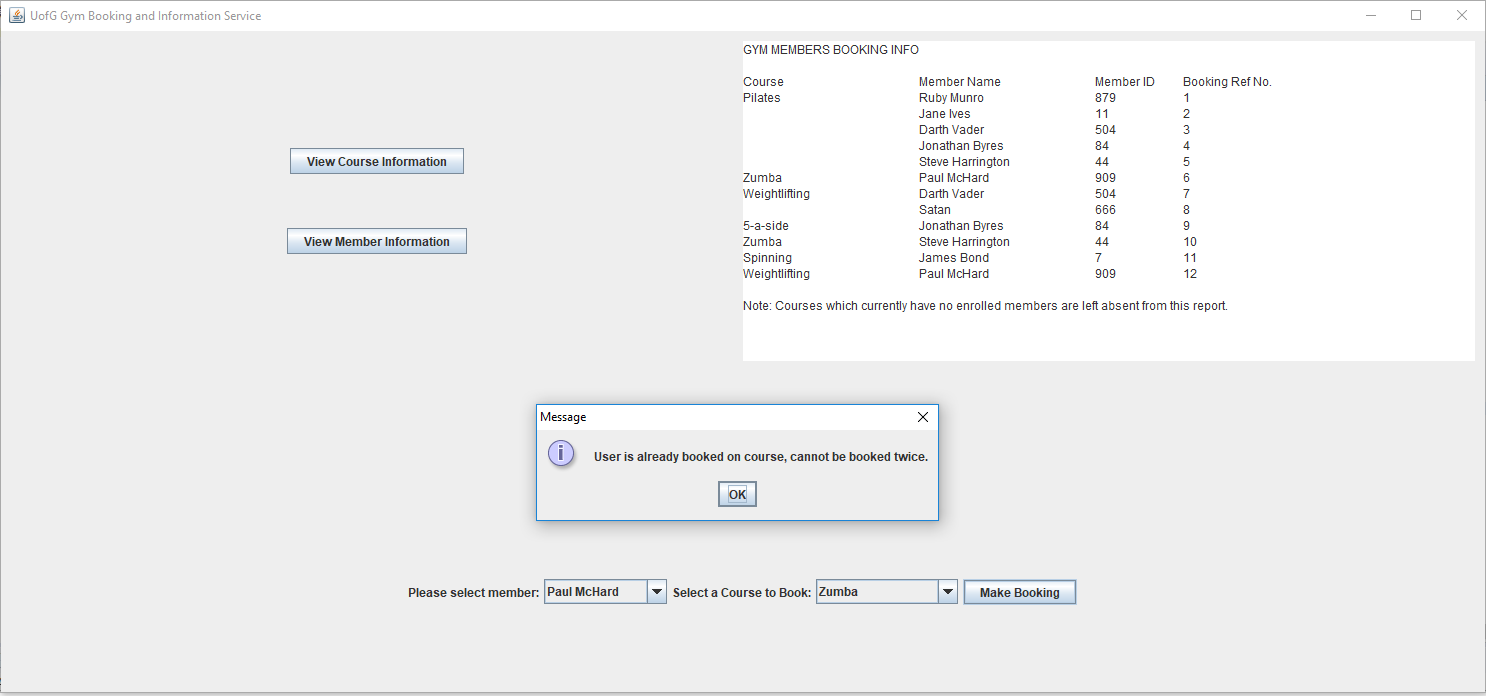
\includegraphics[width=17cm]{fig10}
\caption*{ \textit{Figure 6} }
\end{figure}


\end{document}  